\documentclass{article}
\usepackage{../ml1_submit}
\usepackage{amssymb,amsmath}
\usepackage{graphicx}

% please submit the corresponding pdf by email to
% homework@brml.de, and write "homework sheet xx" in the 
% title.  No more, no less!  (Instead of xx, however,
% put the decimal number of the homework sheet.)

% Please update the following line, only change XX to the homework
% sheet number
\title{homework sheet 06}


\author{
\name{Marco Seravalli}\\
\imat{03626387}\\
\email{marco.seravalli@tum.de}
\And
\name{Nikola Tchipev} \\
\imat{03625168}\\
\email{n.tchipev@tum.de}
}

% The \author macro works with any number of authors. There are two commands
% used to separate the names and addresses of multiple authors: \And and \AND.
%
% Using \And between authors leaves it to \LaTeX{} to determine where to break
% the lines. Using \AND forces a linebreak at that point. So, if \LaTeX{}
% puts 3 of 4 authors names on the first line, and the last on the second
% line, try using \AND instead of \And before the third author name.



\begin{document}
\maketitle

\newpage
\section{Probability Theory}


\subsection*{Problem 1}
First we note that 
\[F_Y(y) = \begin{cases}
            0 & \text{for } y\leq 0 \\
            1 & \text{for } y\geq 1
           \end{cases}
\]

In $[0,1]$, we can say that $F_Y(y)$ is differentiable, strictly positive and strictly increasing, because it is
the integral of the strictly increasing continuous and positive function $F_X(x)$. Furthermore, we can say that
\[ f_Y(y) = \frac{dF_Y}{dy} = \begin{cases}
                                0 & \text{for } y\leq 0 \\
                                0 & \text{for } y\geq 1
                               \end{cases}
\] and that $f_Y(y)$ is positive and continuous on $[0,1]$.


\subsection*{Problem 2}

Show that the sum of two independent random Gaussian variables $X_{1}$,
$X_{2}$ is a Gaussian. \\
We can define every Gaussian random variable $X\sim\mathcal{N}(u,\Sigma)$
using a linear transformation on 
\[
Z\sim\mathcal{N}(0,I)
\]
\[
X=\mu+LZ
\]
 where $L$ is defined by the Cholesky decomposition as 
 \[
 L=\Sigma L^{-T}
 \]
 Hence $X_{1}$and $X_{2}$ can be defined as

 \[
 X_{1}=\mu_{1}+L_{1}Z
 \]
 \[
 X_{2}=\mu_{2}+L_{2}Z
 \]
  if we now sum these two quantities we obtain a new random variable
      $X_{3}$ and we then obtain
      \[
      X_{3}=(\mu_{1}+\mu_{2})+(L_{1}+L_{2})Z
      \]
       $X_{3}$ is again a random variable with the following distribution
       $X_{3}\sim\mathcal{N}(\mu_{1}+\mu_{2},(L_{1}+L_{2})(L_{1}+L_{2})^{T})$.

\subsection*{Problem 3}

It is sufficient to show that the joint probability density function is equal to the product 
of the individual probability densities:
\[
    f_{Z}(z) = f_X(x)f_Y(y).
\]
A direct calculation yields the result:
\[
    \rho(X,Y) = 0, \textrm{ hence } \Sigma = \begin{pmatrix}
                                               \sigma_x^2 & 0   \\
                                               0          & \sigma_y^2
                                             \end{pmatrix}
\]

\[
    \textrm{ and } \Sigma^{-1} = \begin{pmatrix}
                                   \sigma_x^{-2} & 0   \\
                                   0          & \sigma_y^{-2}
                                 \end{pmatrix}
\]
Also, $\det\Sigma = \sigma_x^2 \sigma_y^2$. Now, since $Z=(X,Y)$ is bivariate, we know $f_Z(x,y)$:
\begin{eqnarray*}
    f_Z(z) &=& \frac{1}{2\pi\sqrt{|\Sigma|}} \exp\left(-\frac{1}{2}(z-\mu)^T\Sigma^{-1}(z-\mu)\right)\\
           &=& \frac{1}{2\pi\sigma_x \sigma_y} \exp\left(-\frac{1}{2} \begin{pmatrix}x-\mu_x \\ y-\mu_y\end{pmatrix}^T \begin{pmatrix}\sigma_x^{-2} & 0 \\ 0 & \sigma_y^{-2}\end{pmatrix}\begin{pmatrix}x-\mu_x \\ y-\mu_y\end{pmatrix}\right) \\
           &=& \frac{1}{2\pi\sigma_x \sigma_y} \exp\left(-\frac{1}{2} \left(\left(\frac{x-\mu_x}{\sigma_x}\right)^2 + \left(\frac{y-\mu_y}{\sigma_y}\right)^2\right)\right) \\
           &=& \frac{1}{2\pi\sigma_x \sigma_y} \exp\left(-\frac{1}{2} \left(\frac{x-\mu_x}{\sigma_x}\right)^2 \right)\exp \left( -\frac{1}{2}\left(\frac{y-\mu_y}{\sigma_y}\right)^2\right) \\
           &=& f_X(x)f_Y(y) 
\end{eqnarray*}
Hence, $X$ and $Y$ are independent.


\newpage 
\section{Probability Inequalities}
\subsection{Markov Inequality}

Let $I_{X > c}$ be the indicator random variable of the event $X > c$:
\[
    I_{X> c} = \begin{cases}
                  1 & \text{if $X > c$,} \\
                  0 & \text{otherwise.}
                  \end{cases}
\]
We then have
\[
    cI_{X> c} = \begin{cases}
                   c & \text{if $X > c$,} \\
                   0 & \text{otherwise,}
                   \end{cases}
\]
and hence $$cI_{X> c} \leq X,$$ since $X$ is non-negative. 
Now, by the monotonicity of the expectation operator we have 
$$E[cI_{X> c}] \leq E[X].$$ Taking linearity of $E$, into account,
we get $$cE[I_{X> c}] \leq E[X].$$

Note that we can compute $E[I_{X> c}]$:
\begin{eqnarray*}
    E[I_{X> c}] &=& \sum_{x}p(x)I_{X> c} \\
                   &=& \sum_{x \leq c}p(x)I_{X> c} + \sum_{x > c}p(x)I_{X> c} \\
                   &=& \sum_{x \leq c}p(x)0 + \sum_{x > c}p(x)1 \\
                   &=& \sum_{x > c}p(x) \\
                   &=& P(X> x).
\end{eqnarray*}
Thus, we arrive at $$ cP(X > x) = cE[I_{X > c}] \leq E[X], $$ and hence
$$ P(X > x) \leq \frac{E[X]}{c}.$$

For the second part, let $X$ be the random variable, describing the number
of ``heads'' out of $n$ coin tosses. Since we are throwing a fair coin, we
clearly have $$ E[X] = \frac{n}{2}.$$ Now we have $c=\frac{3}{4}n$ and by the
Markov inequality we obtain 
\[ 
  P\left(X> \frac{3}{4}n\right) \leq \frac{\frac{n}{2}}{\frac{3}{4}n} 
    = \frac{2}{3}
\]
and $$ P\left(X > \frac{3}{4}n\right)\leq \frac{2}{3}.$$


\subsection{Chebyshev Inequality}
Similarly, let $I_{(X - E[X])^2 > c^2}$ be the indicator random variable of the event $(X - E[X])^2 > c^2$:
\[
    I_{(X - E[X])^2 > c^2} = \begin{cases}
                  1 & \text{if $(X - E[X])^2 > c^2$,} \\
                  0 & \text{otherwise.}
                  \end{cases}
\]
We then have
\[
    c^2I_{(X - E[X])^2 > c^2} = \begin{cases}
                   c^2 & \text{if $(X - E[X])^2 > c^2$,} \\
                   0 & \text{otherwise,}
                   \end{cases}
\]
and hence $$c^2I_{(X - E[X])^2 > c^2} \leq (X - E[X])^2.$$ 
Now, by the monotonicity of the expectation operator we have 
$$E[c^2I_{(X - E[X])^2 > c^2}] \leq E[(X-E[X])^2] = Var[E].$$ Taking linearity of $E$, into account,
we get $$c^2E[I_{(X - E[X])^2 > c^2}] \leq Var[E].$$

Note that we can compute $E[I_{(X - E[X])^2 > c^2}]$:
\begin{eqnarray*}
    E[I_{(X - E[X])^2 > c^2}] &=& \sum_{x}p(x)I_{(X - E[X])^2 > c^2}  \\
                              &=& P\left( (X-E[X])^2 > c^2 \right)    \\
                              &=& P\left( |X-E[X]| > c \right)
\end{eqnarray*}
Thus, we arrive at $$ P(|X-E[X]| > c) \leq \frac{Var[X]}{c^2}.$$

For the second part, let again $X$ be the random variable, describing the 
number of ``heads'' out of $n$ coin tosses. Now, due to the symmetry of the 
problem and the fact that $E[X]=\frac{n}{2}$, we make the following 
observation:
\[ P\left( X > \frac{3}{4}n \right) = P\left( X < \frac{1}{4}n \right).  \]

Thus, 
\begin{eqnarray}
P\left( X > \frac{3}{4}n \right) 
& = & \frac{2P\left(X > \frac{3}{4}n\right)}{2} \\
& = & \frac{P\left(X > \frac{3}{4}n\right) + P\left(X < \frac{1}{4}n\right)}{2} \\
& = & \frac{P\left(\{X > \frac{3}{4}n\} \cup \{X < \frac{1}{4}n\}\right)}{2} \\
& = & \frac{P\left( | X - E[X]| > \frac{1}{4}n \right)}{2}.
\end{eqnarray}

Now, after applying Chebyshev's inequality, we obtain:
\[
  P\left( X > \frac{3}{4}n \right) 
    \leq \frac{Var[X]}{2 \left(\frac{1}{4}n\right)^2}
    = \frac{8Var[X]}{n^2}.
\]

Now we just need the variance:
\begin{eqnarray*}
  Var[X] & = & E[(X-E[X])^2] \\
         & = & \sum_xp(x)\left(x-\frac{n}{2}\right)^2 \\
         & = & \sum_{k=0}^n\frac{\binom{n}{k}}{2^n}\left(k-\frac{n}{2}\right)^2.
\end{eqnarray*}


\subsection{Jensen's Inequality}
The statement is obviously true for $n=1$: 
$$ f(1\cdot x_1) \leq 1\cdot f(x_1)$$ and for $n=2$ since $f$ is convex:
$$ f(\lambda x_1 + (1-\lambda)x_2) \leq \lambda f(x_1) + (1-\lambda)f(x_2),$$
which gives us the base step of the induction.

Now suppose it is true for $n=k$ and consider $n=k+1$:
\begin{eqnarray}
  f\left(\sum_{i=1}^{k+1}\lambda_ix_i\right) 
    &=& f\left(\sum_{i=1}^{k}\lambda_ix_i+\lambda_{k+1}x_{k+1}\right) \\
    &=& f\left((1-\lambda_{k+1})\left(\frac{\sum_{i=1}^{k}\lambda_ix_i}{1-\lambda_{k+1}}\right)+\lambda_{k+1}x_{k+1}\right) \\
    &\leq& (1-\lambda_{k+1})f\left(\sum_{i=1}^k\frac{\lambda_ix_i}{1-\lambda_{k+1}}\right) + \lambda_{k+1}f(x_{k+1}) \\
    &\leq& (1-\lambda_{k+1})f\left(\sum_{i=1}^k\frac{\lambda_i}{1-\lambda_{k+1}}x_i\right) + \lambda_{k+1}f(x_{k+1}) \\
    &\leq& (1-\lambda_{k+1})\left(\sum_{i=1}^k\frac{\lambda_i}{1-\lambda_{k+1}}f(x_i)\right) + \lambda_{k+1}f(x_{k+1}) \\
    &=& \sum_{i=1}^k\lambda_if(x_i) + \lambda_{k+1}f(x_{k+1}) \\
    &=& \sum_{i=1}^{k+1}\lambda_if(x_i).
\end{eqnarray}

In going from (6) to (7) we used the definition of convexity of $f$. 
In going from (7) to (8) we use the fact that 
$$ \sum_{i=1}^k\lambda_i = 1 - \lambda_{k+1}$$ and apply the inductive 
hypothesis for $n=k$.


\newpage 
\section*{3 Random Projections}

\subsection*{Problem 7}

Consider the 1D situation. Then there are only two possible cases:

\begin{itemize}
  \item the vectors $\mathbf{u}$ and $\mathbf{v}$ are parallel\\
Then $h_r(\mathbf{u}) = h_r(\mathbf{v})$ is always fulfiled and 
\[p(h_r(\mathbf{u}) = h_r(\mathbf{v})) = 1-\frac{0}{\pi} = 1\]
  \item the vectors $\mathbf{u}$ and $\mathbf{v}$ are antiparallel\\
Then $h_r(\mathbf{u}) = - h_r(\mathbf{v})$ and 
\[p(h_r(\mathbf{u}) = h_r(\mathbf{v})) = 1-\frac{\pi}{\pi} = 0\]
\end{itemize}

Now suppose we are in 2D. It is sufficient to show that \[p\left(h_r(\mathbf{u}) \neq h_r(\mathbf{v})\right)=\frac{\theta(\mathbf{u}, \mathbf{v})}{\pi}.\] Then \[p\left(h_r(\mathbf{u}) = h_r(\mathbf{v})\right) = 1-p\left(h_r(\mathbf{u}) \neq h_r(\mathbf{v})\right) = 1 - \frac{\theta(\mathbf{u}, \mathbf{v})}{\pi}.\]

Let $u_\perp$, $v_\perp$ be the lines, perpendicular to $\mathbf{u}$ and $\mathbf{v}$, respectively. Then the probability that $h_r(\mathbf{u})$ is not equal to $h_r(\mathbf{u})$ is the same as the probability of choosing any point in the plane, which falls in the shaded region in Fig. \ref{fig:theta}. From simple geometry, the angle between $\mathbf{u_\perp}$ and $\mathbf{v_\perp}$ is equal to $\theta(\mathbf{u,v})$. Thus the probability that a randomly chosen point in the plane falls in the shaded region is equal to $\frac{2\theta}{2\pi}=\frac{\theta}{\pi}$, which we wanted to show.
\begin{figure}[!h]
  \begin{center}
    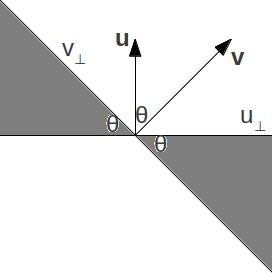
\includegraphics[width=0.25\textwidth]{plots/3.png}
    \caption{2D diagram}
    \label{fig:theta}
  \end{center}
\end{figure}

Now suppose that we are in a higher dimensional space. Then if $\mathbf{u}$ and $\mathbf{v}$ are not parallel or antiparallel (in which case we come down to the same calculation as in 1D, which we already showed), they define a unique plane that contains both of them. It is sufficient to consider the projection of $\mathbf{r}$ onto that plane and whether it lies in the same shaded region as in 2D, hence the problem is reduced to the 2D case.



\newpage 
\section{The preceptron}

\subsection*{Problem 5}
\[
w_{k+1}=\begin{cases}
w_{k}+x_{k} & if\, t_{k}=+1\\
w_{k}-x_{k} & if\, t_{k}=-1
\end{cases}
\]
\[
b_{k+1}=\begin{cases}
b_{k}+1_{k} & if\, t_{k}=+1\\
b_{k}-1_{k} & if\, t_{k}=-1
\end{cases}
\]


\subsection*{Problem 7}
\[
\tilde{w}^{T}w_{k}=\tilde{w}^{T}\left(w_{k-1}+t_{k-1}x_{k-1}\right)=\tilde{w}^{T}\left(w_{k-2}+t_{k-2}x_{k-2}+t_{k-1}x_{k-1}\right)
\]
\[
\tilde{w}^{T}w_{k}=\tilde{w}^{T}\sum_{i=0}^{k-1}t_{i}x_{i}
\]
\[
\tilde{w}^{T}w_{k}=\sum_{i=0}^{k-1}t_{i}\tilde{w}^{T}x_{i}
\]
by knowing that $t_{i}\tilde{w}^{T}x_{i}\geq \gamma$ we can assert
the following
\[
\tilde{w}^{T}w_{k}=\sum_{i=0}^{k-1}t_{i}\tilde{w}^{T}x_{i} \geq \sum_{i=0}^{k-1}\gamma = k\gamma
\]


\subsection*{Problem 8}
\[
\left\Vert w_{k}\right\Vert ^{2}<kR^{2}
\]
from problem 7 we know that $w_{k}=\sum_{i=0}^{k-1}t_{i}x_{i}$ hence
we can write 
\[
\left\Vert \sum_{i=0}^{k-1}t_{i}x_{i}\right\Vert ^{2} \leq kR^{2}
\]
by using the triangle inequality
$\left|A+B\right|\leq\left|A\right|+\left|B\right|$
we can be sure that $\left\Vert \sum_{i=0}^{k-1}t_{i}x_{i}\right\Vert ^{2}$
is smaller or equal than $kR^{2}$.



\subsection*{Problem 9}
We can rewrite $\tilde{w}^{T}w_{k}$ by using problem 7 as 
\[
\left\Vert \tilde{w^{T}}\right\Vert \left\Vert w_{k}\right\Vert
cos(\alpha)=\left\Vert \tilde{w^{T}}\right\Vert \left\Vert
\sum_{i=0}^{k-1}t_{i}x_{i}\right\Vert cos(\alpha)
\]
from problem 7 we know that $\tilde{w}^{T}w_{k}\geq k\gamma$ then
\[
k\gamma\leq\left\Vert \tilde{w^{T}}\right\Vert \left\Vert
\sum_{i=0}^{k-1}t_{i}x_{i}\right\Vert cos(\alpha)
\]
from problem 8 we have $\left\Vert w_{k}\right\Vert ^{2}<kR^{2}$,
thus 
\[
k\gamma\leq\left\Vert \tilde{w^{T}}\right\Vert \left\Vert
\sum_{i=0}^{k-1}t_{i}x_{i}\right\Vert cos(\alpha)
\]
\[
\left(k\gamma\right)^{2}\leq\left(\left\Vert \tilde{w^{T}}\right\Vert
\left\Vert \sum_{i=0}^{k-1}t_{i}x_{i}\right\Vert
cos(\alpha)\right)^{2}<\left\Vert \tilde{w^{T}}\right\Vert
^{2}kR^{2}cos^{2}(\alpha)
\]
\[
k\leq\frac{\left\Vert \tilde{w^{T}}\right\Vert
^{2}R^{2}cos^{2}(\alpha)}{\gamma^{2}}\leq\frac{\left\Vert
\tilde{w^{T}}\right\Vert ^{2}R^{2}}{\gamma^{2}}
\]
  
\newpage
\subsection*{Problem 10}
The data are not separable with the perceptron algorithm because the convex
hulls formed by the points intersect and as it was shown in problem 1 if this 
happens the data are not lineraly separable.
\begin{figure}
\centering{}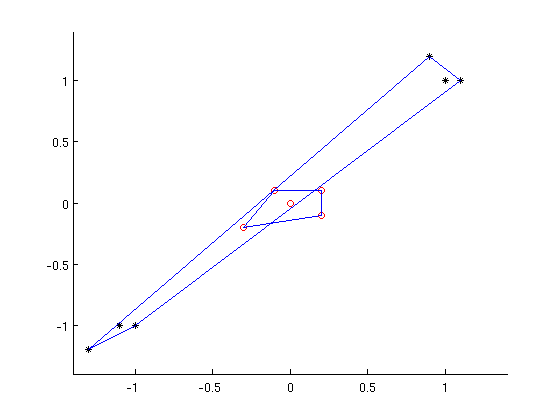
\includegraphics[width=1\textwidth]{plots/10_hull_1}\caption{Hulls}
\end{figure}

\newpage
\subsection*{Problem 11}
The two hulls now do not intersect therefore the two data sets are lineraly
separable
\begin{figure}
\centering{}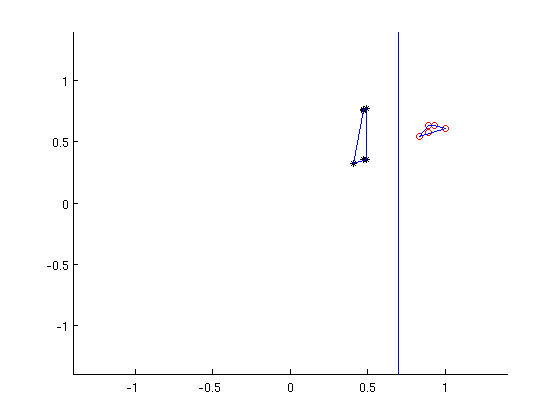
\includegraphics[width=1\textwidth]{plots/10_hull_2}\caption{Hulls}
\end{figure}

\newpage
\subsection*{Problem 6}
\begin{figure}
\centering{}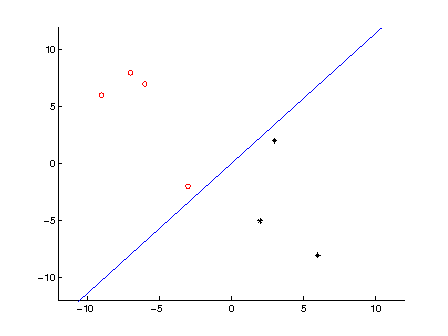
\includegraphics[width=1\textwidth]{plots/6_1}\caption{Problem 6 step 1}
\end{figure}
\begin{figure}
\centering{}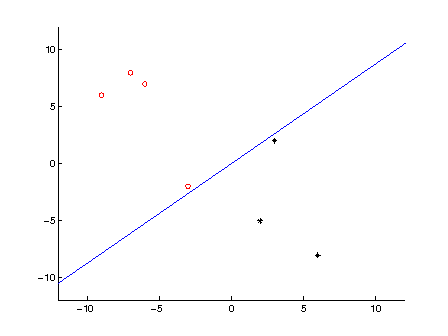
\includegraphics[width=1\textwidth]{plots/6_2}\caption{Problem 6 step 2}
\end{figure}
\begin{figure}
\centering{}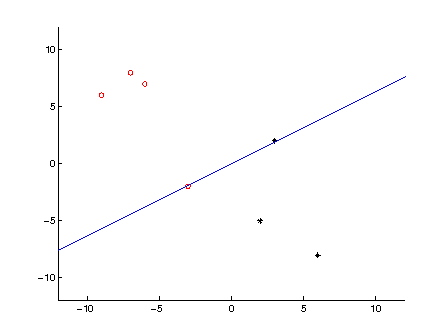
\includegraphics[width=1\textwidth]{plots/6_3}\caption{Problem 6 step 3}
\end{figure}
\begin{figure}
\centering{}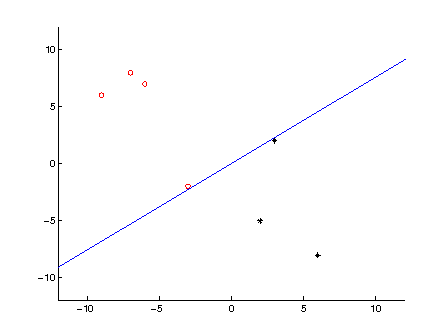
\includegraphics[width=1\textwidth]{plots/6_4}\caption{Problem 6 step 4}
\end{figure}
\begin{figure}
\centering{}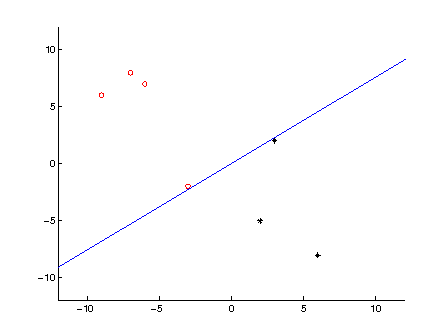
\includegraphics[width=1\textwidth]{plots/6_4}\caption{Problem 6 step 5}
\end{figure}
\begin{figure}
\centering{}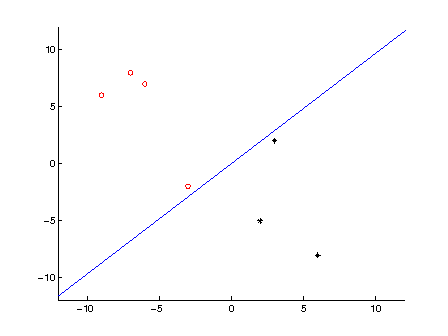
\includegraphics[width=1\textwidth]{plots/6_6}\caption{Problem 6 step 6}
\end{figure}
\begin{figure}
\centering{}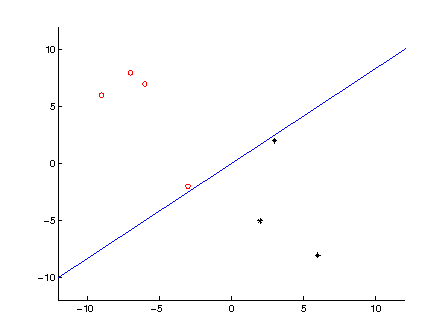
\includegraphics[width=1\textwidth]{plots/6_7}\caption{Problem 6 step 7}
\end{figure}




\end{document}
